% https://tex.stackexchange.com/questions/180888/tikz-extend-a-line-along-a-path
\documentclass[tikz]{standalone}

\usetikzlibrary{decorations.markings,intersections,calc}

        %%%%                        ---- Use path several times
        %%%%                        ---- thanks to Andrew Stacey
        \makeatletter
        \tikzset{
          use path for main/.code={%
            \tikz@addmode{%
              \expandafter\pgfsyssoftpath@setcurrentpath\csname tikz@intersect@path@name@#1\endcsname
            }%
          },
          use path for actions/.code={%
            \expandafter\def\expandafter\tikz@preactions\expandafter{\tikz@preactions\expandafter\let\expandafter\tikz@actions@path\csname tikz@intersect@path@name@#1\endcsname}%
          },
          use path/.style={%
            use path for main=#1,
            use path for actions=#1,
          }
        }

% #1 premier path               ---- Intersection ----
% #2 second path
% #3 nom des points
\newcommand{\InterSec}[3]{%
\path[name intersections={of=#1 and #2, by=#3, sort by=#1,total=\t}]
\pgfextra{\xdef\InterNb{\t}}; }

\begin{document}
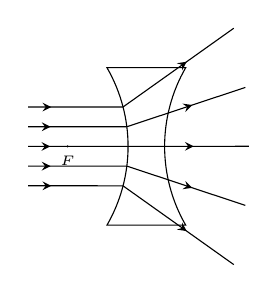
\begin{tikzpicture}
  \pgfmathsetmacro{\lH}{1}
  \pgfmathsetmacro{\lR}{2}
  \pgfmathsetmacro{\sA}{asin(\lH/\lR)}
  \pgfmathsetmacro{\base}{1}
  \pgfmathsetmacro{\xshi}{\base/2}

  \draw[yshift = -2cm, xshift = -\xshi cm,name path=lens] (0, \lH cm)
  arc[start angle = -\sA, delta angle = 2*\sA, radius = \lR cm] --
  +(\base cm, 0)
  arc[start angle = 180 - \sA, delta angle = 2*\sA, radius = \lR cm]
   -- cycle;
  \fill[fill = black] (-1cm, 0) coordinate (F) circle[radius = 0.015cm] node[below,
  font = \tiny] {$F$}; 

  \begin{scope}[decoration = {
      markings,
      mark = at position 0.1 with {\arrow{stealth}},
      mark = at position 0.75 with {\arrow{stealth}}
    }
    ]
%   \foreach \y  in {0.5, 0.25, 0, -0.25, -0.5}{
%     \draw[postaction = decorate] (-1.5cm, \y cm) -- (0, \y cm)
%     coordinate (A) 
%     -- ($(F)!3!(A)$) ;      
      %extend lines along the path command here;

    \foreach \y  in {0.5, 0.25, 0, -0.25, -0.5}{
      \path[name path=ray] (-1.5cm, \y cm) -- (0, \y cm) ;
      \InterSec{ray}{lens}{A}
      \draw[postaction = decorate] (-1.5cm, \y cm) -- (A) -- ($(F)!3!(A)$) ;      

    }
  \end{scope}

\end{tikzpicture}
\end{document}

%%% Local Variables:
%%% mode: latex
%%% TeX-master: t
%%% End:
